\section{线性松弛}
\label{sec:lp-relaxation}

产品如果只能整批生产，变量就必须取整数。于是要问：去掉整数要求之后，连续问题的解和最优值能告诉我们整数问题的什么？回答分三层：最优值总能给出一个界；在特殊的矩阵结构下，顶点自动是整数；一般情形下，连续解还要经过专门论证的处理，才能变成原问题的可行解。

\paragraph{整数问题与它的松弛}
在标准型或不等式形式的线性规划上再要求变量取整数，就得到\term{整数线性规划}（integer linear programming）。设
\begin{equation}
 p_{\mathrm{I}}=\min\{\bm{c}^\top\bm{x}:\bm{x}\in\bm{C},\ \bm{x}\in\mathbb{Z}^n\},
 \qquad
 p_{\mathrm{R}}=\min\{\bm{c}^\top\bm{x}:\bm{x}\in\bm{C}\}.
 \label{eq:lp-relaxation-values}
\end{equation}
去掉整数要求后的问题称为原问题的\term{线性松弛}（linear relaxation）。这里的$\bm{C}$可以是任何多面体。

松弛扩大了可行集，最小化时最优值只会变小或不变。这是下面定理的全部内容，也是松弛提供的最基本的信息。

\begin{theorem}[松弛给出下界]
 \label{thm:lp-relaxation-bound}
 若整数问题可行且松弛的最优值有限，则
 \begin{equation}
  p_{\mathrm{R}}\leq p_{\mathrm{I}}.
  \label{eq:lp-relaxation-bound}
 \end{equation}
 若松弛有一个最优解是整数向量，则它也是整数问题的最优解，且等号成立。
\end{theorem}

\begin{proof}
 整数问题的可行点都在$\bm{C}$中，在较大的集合上取最小值不会更大，得到式~\eqref{eq:lp-relaxation-bound}。若松弛的最优解$\bm{x}$是整数向量，它对整数问题可行，于是
 \[
  p_{\mathrm{I}}\leq\bm{c}^\top\bm{x}=p_{\mathrm{R}}.
 \]
 再与式~\eqref{eq:lp-relaxation-bound}合并，等号成立。
\end{proof}

用一个具体的整数问题走一遍。把车间的原料增加到$7$份，利润系数改成$(3,1)$，并要求产量取整数：
\[
 \max\ 3x_1+x_2\quad\text{s.t.}\quad x_1+x_2\leq4,\quad2x_1+x_2\leq7,\quad\bm{x}\geq\bm{0},\quad\bm{x}\in\mathbb{Z}^2.
\]
松弛的四个顶点是$(0,0),(7/2,0),(3,1),(0,4)$，对应的利润依次是
\[
 0,\qquad\frac{21}{2},\qquad10,\qquad4.
\]
所以松弛的最优解是$(7/2,0)$，最优利润$21/2$。按$x_1$的取值逐个比较可行的整数点，$x_1$固定时$x_2$取最大，四种情形的利润依次是
\[
 x_1=0:\ 4,\qquad x_1=1:\ 6,\qquad x_1=2:\ 8,\qquad x_1=3:\ 10.
\]
$x_1\geq4$时原料不够，所以整数问题的最优解是$(3,1)$，利润$10$。这里是最大化，松弛给出的是上界，写成最小化$-3x_1-x_2$时，就是$p_{\mathrm{R}}=-21/2\leq-10=p_{\mathrm{I}}$。

\paragraph{舍入不是免费的}
最直接的想法是把松弛解舍入成整数。图~\ref{fig:lp-rounding}显示这个想法的问题。$(7/2,0)$向上取整得到$(4,0)$，用掉$8$份原料，不可行。向下取整得到$(3,0)$，可行，利润只有$9$，也不是最优。真正的最优解$(3,1)$在$x_2$上离松弛解差了一整个单位，它不是任何一种舍入的结果。

\begin{BookInlineFigure}
 \centering
 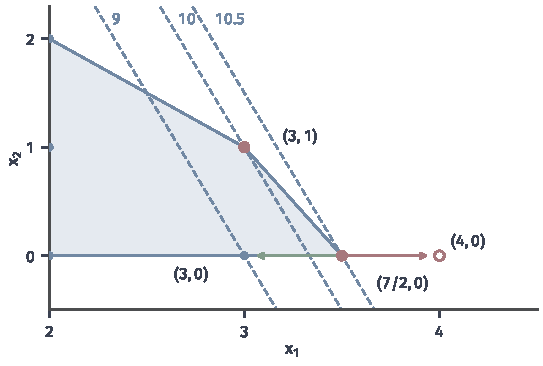
\includegraphics[width=92mm]{figures/05-optimization/01-linear-programming/matplotlib/lp-rounding/figure.pdf}
 \caption{舍入松弛解。蓝点是可行的整数点，蓝色虚线是利润$9$、$10$、$10.5$的等值线。松弛最优解$(7/2,0)$（红点，位于右下顶点）向右舍入到不可行的$(4,0)$（红色空心点），向左舍入到利润只有$9$的$(3,0)$；整数最优解是红点$(3,1)$。}
 \label{fig:lp-rounding}
\end{BookInlineFigure}

松弛最优值虽然不直接给出解，却给出了一个证明的工具。目标系数和变量都是整数时，$p_{\mathrm{I}}$也是整数，所以下界可以向上取整：
\[
 p_{\mathrm{I}}\geq\lceil p_{\mathrm{R}}\rceil=\Bigl\lceil-\frac{21}{2}\Bigr\rceil=-10.
\]
而$(3,1)$的目标值恰好是$-10$，这就证明了它是最优的，不需要枚举。一般情形下，松弛最优值和某个可行整数点的目标值夹出的区间，是对整数最优值的一个估计，这个区间的宽度取决于松弛有多紧。

$p_{\mathrm{I}}-p_{\mathrm{R}}$称为这个实例的\term{整数间隙}（integrality gap），这里是$1/2$。整数间隙衡量松弛对原问题的逼近程度，与求解松弛的算法无关。

\paragraph{整数顶点：全幺模}
既然线性规划的最优解可以在顶点取得，顶点若都是整数，整数约束就没有额外的代价。对比图~\ref{fig:lp-integer-hull}的两个多面体，它们的矩阵相同，右端不同：原料为$6$时四个顶点都是整数，原料为$7$时出现了分数顶点$(7/2,0)$。顶点是否整数，到底由什么决定？

\begin{BookInlineFigure}
 \centering
 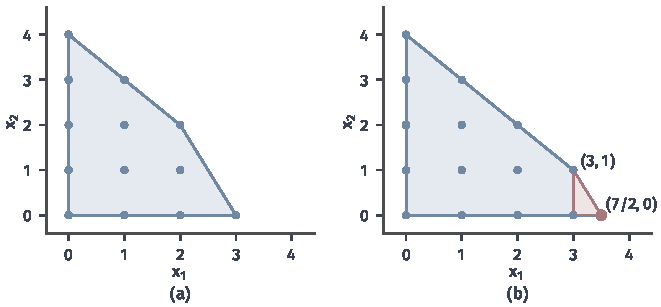
\includegraphics[width=112mm]{figures/05-optimization/01-linear-programming/matplotlib/lp-integer-hull/figure.pdf}
 \caption{相同的约束矩阵，不同的右端。蓝点是可行的整数点。(a)~原料为$6$，四个顶点都是整数。(b)~原料为$7$，右下顶点$(7/2,0)$是分数，红色小三角形是松弛比全体整数点的凸包多出的部分。}
 \label{fig:lp-integer-hull}
\end{BookInlineFigure}

答案在定义基本解的式~\eqref{eq:lp-basic-solution}里。由Cramer法则，
\[
 (\bm{x}_B)_i=\frac{\det\bm{A}_B^{(i)}}{\det\bm{A}_B},
\]
其中$\bm{A}_B^{(i)}$是把$\bm{A}_B$的第$i$列换成$\bm{b}$得到的矩阵。$\bm{A}$和$\bm{b}$都是整数时分子是整数，分数只能来自分母。如果基矩阵的行列式总是$\pm1$，顶点就一定是整数。图~\ref{fig:lp-integer-hull}(b)的分数顶点来自基$\{1,3\}$，它的行列式是$-2$，分母是$2$，而$7$是奇数；$b_2=6$时$6/2$仍是整数，分母恰好被消去。

\begin{definition}[全幺模矩阵]
 \label{def:lp-tu}
 若矩阵$\bm{A}$的每个方子矩阵的行列式都属于$\{0,1,-1\}$，就称$\bm{A}$是\term{全幺模矩阵}（totally unimodular matrix）。
\end{definition}

特别地，全幺模矩阵的元素都只能是$0,\pm1$。这个条件对所有方子矩阵提出要求，而不只是对基矩阵，这样它才能在加松弛变量、删冗余行这些改写后保持下来。

\begin{theorem}[全幺模与整数顶点]
 \label{thm:lp-tu-integral}
 设$\bm{A}$满行秩且全幺模，$\bm{b}$是整数向量。则$\bm{C}$的每个基本可行解都是整数向量。若问题可行且最优值有限，则存在整数最优解，从而
 \begin{equation}
  p_{\mathrm{I}}=p_{\mathrm{R}}.
  \label{eq:lp-tu-exact}
 \end{equation}
\end{theorem}

\begin{proof}
 任取基$B$。$\bm{A}_B$是可逆的方子矩阵，所以$\det\bm{A}_B=\pm1$。由Cramer法则，$\bm{x}_B$的每个分量都是整数行列式除以$\pm1$，是整数。第二句由定理~\ref{thm:lp-optimal-bfs}和定理~\ref{thm:lp-relaxation-bound}得到。
\end{proof}

不等式形式也可以用。若$\bm{A}$全幺模，则$[\bm{A}\ \ \bm{I}]$也全幺模：它的方子矩阵若含单位矩阵的列，这一列至多有一个非零元，按这一列展开，行列式化成$\bm{A}$的更小子矩阵的行列式，或者为零。于是不等式约束$\bm{A}\bm{x}\leq\bm{b}$，$\bm{x}\geq\bm{0}$在加了松弛变量之后满足定理的条件，变量的整数上界也可以同样处理。

定理的每个条件都起作用。$\bm{A}$全幺模但$\bm{b}$不是整数时，顶点就不是整数，例如$x_1\leq1/2$，$x_1\geq0$的顶点$1/2$。反过来，全幺模只是充分条件：车间矩阵含元素$2$，不是全幺模的，但$b_2=6$时顶点恰好都是整数。

定理说的是基本可行解，不是所有最优解。图~\ref{fig:lp-optimal-face}(b)那样有整条最优边的情形，边上的点可以不是整数，所以要得到整数解，必须取到顶点。

\paragraph{网络矩阵是全幺模的}
最重要的全幺模矩阵来自有向图。这正是图上的最短路、最大流、最小费用流可以用连续方法求整数解的原因。

\begin{theorem}[关联矩阵全幺模]
 \label{thm:lp-incidence-tu}
 设矩阵的每一列至多有一个$+1$、至多有一个$-1$，其余元素为零。有向图的关联矩阵就是这样的矩阵。这样的矩阵是全幺模的。
\end{theorem}

\begin{proof}
 对方子矩阵$\bm{D}$的阶数$k$归纳。$k=1$时元素属于$\{0,\pm1\}$。设$k>1$，$\bm{D}$的列也满足“至多一个$+1$、至多一个$-1$”，分三种情形。

 若某列全为零，$\det\bm{D}=0$。若某列恰有一个非零元，按这一列展开，$\det\bm{D}$等于$\pm$一个$k-1$阶子矩阵的行列式，由归纳假设属于$\{0,\pm1\}$。若每一列都恰有一个$+1$和一个$-1$，则所有行相加是零向量，$\det\bm{D}=0$。
\end{proof}

网络矩阵~\eqref{eq:lp-network-data}不是满行秩的，删去一行之后仍是全幺模矩阵的子矩阵，定理~\ref{thm:lp-tu-integral}可以使用。所以整数供需量、整数容量的最小费用流问题，线性规划的顶点解就是整数流，这正是第~\ref{sec:lp-duality}节实例中的最短路自动取$0$或$1$的原因。

二部图的情形也可以化成这个定理。把无向边看成两个非零元都是$+1$的列，二部图把顶点分成两侧，把一侧对应的行乘以$-1$，列就有了一个$+1$和一个$-1$，行列式只改变符号，所以二部图的关联矩阵也是全幺模的。这解释了指派问题的连续解为何能取整数，可参考\BookChapterRef{chap:bipartite-matching-assignment}{卷三第6章“二部图匹配与指派”}。

\paragraph{整数点的凸包}
全幺模解决了一类问题，一般情形还可以这样理解。有限个点$\bm{v}_1,\ldots,\bm{v}_k$的凸包是它们全部的加权平均，权重非负且和为$1$。线性目标在凸包上的最小值，等于在这些点上的最小值，因为加权平均不会比最小的项更小。

所以，若能把全体整数可行点的凸包用线性不等式写出来，整数问题就成了线性规划，图~\ref{fig:lp-integer-hull}(a)就是这种幸运的情形，松弛恰好等于这个凸包。图~\ref{fig:lp-integer-hull}(b)中松弛比凸包多了一块，多出来的部分造成了整数间隙。困难在于，一般的整数问题的凸包写不出来，不等式的条数可能随规模急剧增长。

\paragraph{一般情形：分数顶点}
图中只要出现奇圈，上面的论证就失效。考虑三个顶点的完全图（三角形），要选出尽量少的顶点，使每条边至少有一个端点被选中。这称为\term{顶点覆盖}（vertex cover）。用$x_i\in\{0,1\}$表示是否选中顶点$i$，问题是
\begin{equation}
 \min\ x_1+x_2+x_3
 \quad\text{s.t.}\quad x_1+x_2\geq1,\quad x_2+x_3\geq1,\quad x_1+x_3\geq1.
 \label{eq:lp-triangle-cover}
\end{equation}
松弛把$x_i\in\{0,1\}$放宽为$x_i\geq0$。三条约束取等号解出的点是
\[
 \bm{x}=\Bigl(\frac12,\frac12,\frac12\Bigr)^\top,\qquad\text{目标值}\ \frac32.
\]

它确实是松弛的最优解。把三条约束相加，得到$2(x_1+x_2+x_3)\geq3$，这正是取权重$(1/2,1/2,1/2)$的对偶证书，于是$p_{\mathrm{R}}=3/2$。

分数从哪里来？三条约束的系数矩阵是
\[
 \bm{E}=\begin{bmatrix}1&1&0\\0&1&1\\1&0&1\end{bmatrix},\qquad\det\bm{E}=2.
\]
行列式是$2$，所以不是全幺模矩阵，Cramer法则的分母正是$2$。三角形是奇圈，不能分成两侧，二部图的变号办法用不上。

整数问题的最优值是$2$：只选一个顶点时，对边的两端都没被选中，这条边没有被覆盖，所以至少选两个；选两个正好够。图~\ref{fig:lp-triangle-cover}对比了三种取值，这个实例的整数间隙是$2-3/2=1/2$。

\begin{BookInlineFigure}
 \centering
 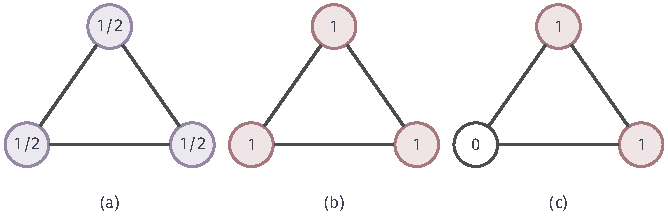
\includegraphics[width=112mm]{figures/05-optimization/01-linear-programming/tikz/lp-triangle-cover/figure.pdf}
 \caption{三角形上的顶点覆盖。圆内的数字是变量取值。(a)~松弛的最优解，三个变量都是$1/2$，目标值$3/2$。(b)~按阈值$1/2$舍入，三个变量都变成$1$，可行，目标值$3$。(c)~整数最优解之一，选两个顶点，目标值$2$。}
 \label{fig:lp-triangle-cover}
\end{BookInlineFigure}

\paragraph{从松弛解恢复可行解}
一般情形下，松弛解未必是整数，需要一个恢复步骤。恢复之后要分别回答两个问题：得到的点可行吗？目标值损失了多少？这两件事都要针对具体的约束结构来证明。前面的车间例子说明，随手舍入可能直接破坏可行性。

顶点覆盖是能够完整论证的例子。设无向图的顶点集为$V$，边集为$E$，顶点权重$w_i\geq0$。求解松弛
\[
 \min\ \sum_{i\in V}w_ix_i\quad\text{s.t.}\quad x_i+x_j\geq1\ \ (\{i,j\}\in E),\quad\bm{x}\geq\bm{0},
\]
得到最优解$\bm{x}^\star$，然后按阈值舍入：$x_i^\star\geq1/2$时取$\widehat{x}_i=1$，否则取$\widehat{x}_i=0$。

\begin{theorem}[顶点覆盖的阈值舍入]
 \label{thm:lp-cover-rounding}
 上述$\widehat{\bm{x}}$是可行的顶点覆盖，并且
 \begin{equation}
  \sum_{i\in V}w_i\widehat{x}_i\leq2\,p_{\mathrm{R}}\leq2\,p_{\mathrm{I}}.
  \label{eq:lp-cover-rounding}
 \end{equation}
\end{theorem}

\begin{proof}
 可行性：对每条边$\{i,j\}$，$x_i^\star+x_j^\star\geq1$，两个数中至少有一个不小于$1/2$，相应的$\widehat{x}$取$1$，这条边被覆盖。

 目标值：按舍入规则，每个$i$都满足$\widehat{x}_i\leq2x_i^\star$。权重非负，逐项相加，得到
 \[
  \sum_{i\in V}w_i\widehat{x}_i\leq2\sum_{i\in V}w_ix_i^\star=2p_{\mathrm{R}}.
 \]
 第二个不等号是定理~\ref{thm:lp-relaxation-bound}。
\end{proof}

三角形上这个界是$3\leq2\cdot\frac32$，等号成立，实际的最优值是$2$。系数$2$不能靠这种比较再改善。在$k$个顶点的完全图上，取单位权重，把全部边的约束相加，每个顶点出现$k-1$次，得到
\[
 (k-1)\sum_ix_i\geq\frac{k(k-1)}{2},\qquad\text{即}\qquad\sum_ix_i\geq\frac{k}{2}.
\]
全取$1/2$可以达到这个下界，松弛最优值是$k/2$。整数解至多有一个顶点不选，否则两个不选的顶点之间的边没被覆盖，所以整数最优值是$k-1$。两者之比随$k$增大趋于$2$。

这个定理的两个结论都依赖顶点覆盖的结构：可行性靠“两个数之和不小于$1$”，误差靠权重非负。换一种约束，例如前面车间的问题，同样的阈值可能得到不可行的点。所以，线性松弛本身只提供界和一个出发点，恢复原问题可行解的方法要逐类设计，并单独论证可行性和误差保证。

松弛的界不紧或者恢复的解不够好时，还可以继续加入有效的不等式来收紧松弛，或者把问题分成子问题分别求解。这类方法都要反复求解线性规划，第~\ref{chap:simplex-method}章将说明怎样在约束增加之后，利用已有的基接着求解。
